\chapter{测度的密度}
\label{chap:measure-densities}
\label{chap:densities-change-of-measure}

区间$[0,1]$上的质量可以均匀分布，也可以向右端堆积，还可以有一部分集中在一个点上。用长度作参照，均匀分布的质量处处是长度的同一个倍数，向右堆积的质量在右端是长度的更大倍数，而点上的质量无论乘以什么倍数都不能从长度得到，因为单点的长度为零。本章研究这种“相对于参考测度的倍数”：一个测度何时能写成另一个测度的加权积分，权重函数怎样计算，以及有了权重之后积分怎样改写。

回答从测度之间最粗的关系开始。第一节只看零测集：参考测度认为可以忽略的集合，目标测度是否也忽略；两个测度能否被一个可测集合完全分开。第二节先从“给定权重得到测度”的方向定义相对密度，再用Radon–Nikodym定理说明，在$\sigma$有限条件下绝对连续恰好保证密度存在，并且密度几乎处处唯一。第三节把一般的测度分成能用密度表示的部分与和参考测度相互奇异的部分，并在实轴上把后者进一步分成点质量与奇异连续质量。

有了密度，第四节建立运算规则：换测度公式把对目标测度的积分改写成对参考测度的加权积分，相对同一参考的密度可以线性组合，逐次更换参考时密度相乘，两个测度等价时密度可以取倒数。第五节回到具体对象，由点质量之比计算离散测度的密度，由累积函数的导数计算实轴测度的密度，并说明导数为何不能恢复点质量与奇异连续质量。

本章的测度都定义在同一个可测空间上，所用的测度构造、有符号测度的Hahn与Jordan分解来自第~\ref{chap:measure}章，积分、单调收敛定理与绝对连续函数的微积分基本定理来自第~\ref{chap:integration}章。点经过映射从一个空间移到另一个空间时质量怎样转移，以及相应的坐标换元，是第~\ref{chap:pushforward-measures}章的内容。

\section{绝对连续与相互奇异}
\label{sec:dens-ac-singular}

同一个可测空间上可以放很多测度：长度、点质量、计数测度以及它们的加权和。比较两个测度时，最粗也最基本的信息是它们怎样对待“可以忽略的集合”。本节固定可测空间$(X,\mathcal A)$上的两个非负测度，一个作为参考，一个作为要描述的目标，只用集合上的测度值回答两个问题：参考测度忽略的集合，目标测度是否也忽略；两个测度的质量能否分别集中在两个互不相交的可测集合上。这两种关系都由集合定义，不涉及积分，也还没有任何密度函数。

记号约定：$\lambda$表示实轴上的Lebesgue测度；对可测集$E$，$\lambda|_E(A)=\lambda(A\cap E)$表示把$\lambda$限制到$E$上得到的测度，它仍定义在整条实轴上；$\delta_a$表示位于点$a$的单位点质量，$\delta_a(A)=1$当且仅当$a\in A$。

\subsection{测度的绝对连续}
\label{sec:dens-absolute-continuity}

设$\mu$是我们用来判断“哪些集合可以忽略”的参考测度。若凡是$\mu$忽略的集合，目标测度$\nu$也一律忽略，那么在$\mu$下几乎处处成立的结论，在$\nu$下也几乎处处成立。下一节会看到，这正是用$\mu$的加权积分表示$\nu$的前提。

\begin{definition}[测度的绝对连续与等价]
\label{def:dens-absolute-continuity}
设$\mu,\nu$是$(X,\mathcal A)$上的非负测度。若对每个$A\in\mathcal A$，
\[
\mu(A)=0\ \Longrightarrow\ \nu(A)=0 ,
\]
就称$\nu$相对于$\mu$\term{绝对连续}（absolutely continuous），记作$\nu\ll\mu$。若$\nu\ll\mu$与$\mu\ll\nu$同时成立，就称$\mu$与$\nu$是\term{等价测度}（equivalent measures），记作$\mu\sim\nu$。
\end{definition}

关系有方向。$\nu\ll\mu$说的是$\mu$的零测集族包含在$\nu$的零测集族之中，参考测度写在右边。它只比较测度值是否为零，不比较非零值的大小；等价也只说明两个测度认可同一族零测集，不说明它们给同一集合相同的值。

\begin{example}[两点空间上的单向关系]
\label{ex:dens-two-point}
取$X=\{0,1\}$，$\mathcal A$为全部子集，$\mu=\delta_0+\delta_1$，$\nu=\delta_0$。$\mu$给每个单点质量$1$，零测集只有空集，所以条件“$\mu(A)=0\Rightarrow\nu(A)=0$”只需对$A=\varnothing$检查，$\nu\ll\mu$成立。反方向不成立：$\nu(\{1\})=0$，而$\mu(\{1\})=1$。再取$\rho=2\delta_0+5\delta_1$，它与$\mu$的零测集都只有空集，于是$\rho\sim\mu$，尽管$\rho(\{1\})=5\neq\mu(\{1\})$。
\end{example}

参考测度不必是Lebesgue测度。上例中参考测度是离散的，零测集由“哪些点没有质量”决定。在实轴上以$\lambda$为参考时，零测集包含所有单点和可数集，因此容易只拿单点来检验。单点检查足以否定$\delta_0\ll\lambda$：$\lambda(\{0\})=0$，而$\delta_0(\{0\})=1$。但单点检查一般不够。

\begin{example}[区间上的连续质量]
\label{ex:dens-two-intervals}
比较$\lambda|_{[0,1]}$与$\lambda|_{[2,3]}$。两者给每个单点的质量都是零，单点完全看不出差别；然而$\lambda|_{[2,3]}([0,1])=0$，$\lambda|_{[0,1]}([0,1])=1$，所以$\lambda|_{[0,1]}\ll\lambda|_{[2,3]}$不成立，反方向同理。另一方面$\lambda|_{[0,1]}\ll\lambda$：$\lambda(A)=0$推出$\lambda(A\cap[0,1])=0$。原因在于$[0,1]$不可数，可数可加性不允许把它的质量拆成单点质量之和；定义要求对每个可测集检查。图~\ref{fig:dens-absolute-continuity}对照了本例与上一例。
\end{example}

\begin{figure}[!htbp]
  \centering
  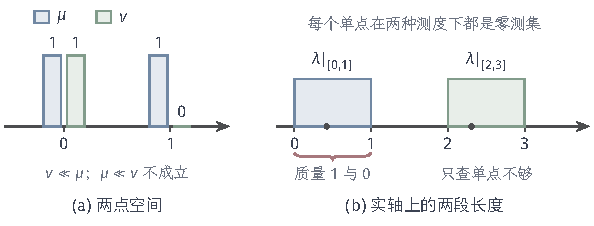
\includegraphics[width=100.669mm]{figures/02-abstract-mathematics/01-metric-and-measure/tikz/c2-absolute-continuity/figure.pdf}
  \caption{绝对连续比较的是零测集。(a)两点空间上$\mu=\delta_0+\delta_1$（蓝）与$\nu=\delta_0$（绿）：$\mu$只把空集看作零测集，所以$\nu\ll\mu$；$\nu$在点$1$的质量为零而$\mu$不为零，所以反向不成立。(b)$\lambda|_{[0,1]}$（蓝）与$\lambda|_{[2,3]}$（绿）在每个单点上都为零，但在$[0,1]$上分别为$1$与$0$，两者互不绝对连续。}
  \label{fig:dens-absolute-continuity}
\end{figure}

\paragraph{与函数的绝对连续}
名称“绝对连续”在第~\ref{chap:integration}章已经用于函数：区间上的函数若在总长度很小的有限个小区间上增量之和也很小，就称它绝对连续。两个概念分别定义，联系要等到第~\ref{sec:dens-cumulative-density}小节才说明：单调函数绝对连续，当且仅当它的增量所产生的测度相对于$\lambda$绝对连续。测度的名称也与“小推出小”有关：若$\nu$有限，则$\nu\ll\mu$等价于对每个$\varepsilon>0$存在$\delta>0$，使$\mu(A)<\delta$推出$\nu(A)<\varepsilon$。本章不使用这一刻画，这里不给出证明。

\subsection{测度的相互奇异}
\label{sec:dens-mutual-singularity}

绝对连续描述的是“参考测度忽略的地方，目标测度也忽略”。与它相对的另一种极端是两个测度各自待在对方忽略的区域里，质量完全不重叠。若$\nu(X\setminus N)=0$，就说$\nu$\emph{集中}在可测集$N$上。

\begin{definition}[相互奇异]
\label{def:dens-mutual-singularity}
设$\mu,\nu$是$(X,\mathcal A)$上的非负测度。若存在$N\in\mathcal A$，使
\[
\mu(N)=0,\qquad\nu(X\setminus N)=0 ,
\]
就称$\mu$与$\nu$\term{相互奇异}（mutually singular），记作$\mu\perp\nu$。
\end{definition}

定义对两个测度是对称的：令$N'=X\setminus N$，则$\nu(N')=0$且$\mu(X\setminus N')=0$，同一关系从$\nu$的角度看就是用补集作分割。直观地说，$X$被一个可测集合分成两块，$\nu$的全部质量在$N$中，$\mu$的全部质量在$X\setminus N$中。在实轴上取$\mu=\lambda|_{[0,1]}$，$\nu=\tfrac12\delta_{1/2}$，$N=\{1/2\}$，则$\mu(N)=0$，$\nu(\mathbb R\setminus N)=0$，所以$\mu\perp\nu$。点$1/2$位于区间内部，相互奇异并不要求两种质量在位置上分开。

两种关系检查的是不同的事。$\nu\ll\mu$问的是$\mu$零测集上有没有$\nu$质量；$\nu\perp\mu$问的是$\nu$能否全部放进一个$\mu$零测集。二者几乎不能同时成立：若$\nu\ll\mu$且$\nu\perp\mu$，取定义中的$N$，则$\mu(N)=0$推出$\nu(N)=0$，又$\nu(X\setminus N)=0$，所以$\nu(X)=0$，$\nu$是零测度。一般的测度两种关系都不满足，例如$\lambda|_{[0,1]}+\delta_2$相对于$\lambda$，第~\ref{sec:dens-decomposition}节将把它拆成满足两种关系的两部分。

\paragraph{集中集合与闭支撑}
在实轴或$\mathbb R^d$上，“相互奇异”很容易被想象成两团质量隔着一段距离。为了说明这种想象不对，先定义Borel测度$\mu$的\term{闭支撑}（support of a measure）：它是这样一些点$x$的集合，$x$的每个开邻域都有正的$\mu$质量。闭支撑的补集是所有$\mu$零测开集之并，因而闭支撑是闭集。$\lambda|_{[0,1]}$的闭支撑是$[0,1]$，$\delta_{1/2}$的闭支撑是$\{1/2\}$，两者相交，测度却相互奇异。

\begin{example}[闭支撑相同而相互奇异]
\label{ex:dens-rationals}
设$(q_n)_{n\geq1}$列举全部有理数，令
\[
\mu=\sum_{n=1}^\infty2^{-n}\delta_{q_n},\qquad\nu=\sum_{n=1}^\infty2^{-n}\delta_{q_n+\sqrt2},
\]
两者都是总质量为$1$的有限测度。$\mu$集中在$\mathbb Q$上，$\nu$集中在$\mathbb Q+\sqrt2$上。这两个集合不相交：若$q=q'+\sqrt2$，则$\sqrt2=q-q'$是有理数，矛盾。取$N=\mathbb Q+\sqrt2$，有$\mu(N)=0$，$\nu(\mathbb R\setminus N)=0$，所以$\mu\perp\nu$。

另一方面，$\mathbb Q$与$\mathbb Q+\sqrt2$都在实轴上稠密，每个非空开区间中两者都有点，所以两个测度在每个非空开区间上都有正质量，闭支撑都是整条实轴。图~\ref{fig:dens-mutually-singular}画出了两组点中的前几个，它们彼此交错。
\end{example}

\begin{figure}[!htbp]
  \centering
  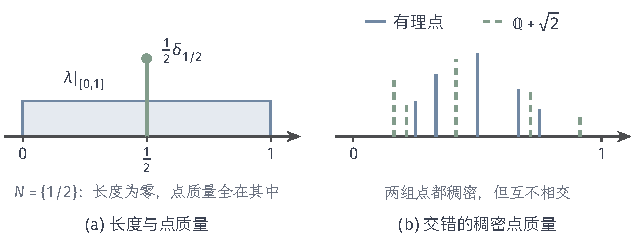
\includegraphics[width=107.668mm]{figures/02-abstract-mathematics/01-metric-and-measure/tikz/c2-mutually-singular/figure.pdf}
  \caption{相互奇异是可测集合上的分离。(a)$\lambda|_{[0,1]}$与$\tfrac12\delta_{1/2}$相互奇异，分离集$N=\{1/2\}$位于区间内部。(b)$\mu=\sum_n2^{-n}\delta_{q_n}$集中在有理点上（蓝色实线），$\nu=\sum_n2^{-n}\delta_{q_n+\sqrt2}$集中在$\mathbb Q+\sqrt2$上（绿色虚线）；图中只画出$[0,1]$内各几个点，线高仅示意权重递减。两组点在每个开区间中都出现，但互不相交，所以$\mu\perp\nu$。}
  \label{fig:dens-mutually-singular}
\end{figure}

这个例子说明，判断相互奇异要找可测的集中集合，而不是看闭支撑是否相交。反方向的蕴含是成立的：若两个闭支撑不相交，取$N$为$\nu$的闭支撑，则$\nu(X\setminus N)=0$：闭支撑的补集中每点都落在某个中心与半径均为有理数、且含于一个$\nu$零测开集的球内，这样的球只有可数个，所以补集是可数个$\nu$零测集之并，而$N$落在$\mu$闭支撑的补集中，$\mu(N)=0$。所以闭支撑不交是相互奇异的充分条件，不是必要条件。顺带一提，上例中的$\mu,\nu$都集中在可数集上，因而都与$\lambda$相互奇异。

\section{相对密度}
\label{sec:dens-relative-density}

绝对连续只是一个关于零测集的条件，它没有给出任何函数。本节从相反的方向进入：先给定参考测度和一个非负权重，用积分产生一个新测度，并把权重称为新测度的相对密度，这一方向不需要任何条件。然后问，给定两个测度，能否找到这样的权重。Radon–Nikodym定理回答，在$\sigma$有限的条件下，绝对连续恰好是所需的条件，而且权重在参考测度几乎处处的意义下唯一。

\subsection{由密度生成测度}
\label{sec:dens-weighted-measure}

给定参考测度，怎样用一个权重函数得到新测度？先在有限点集上看清乘数的含义，再用积分把它推广到一般测度，最后说明权重只在几乎处处意义下确定。

\paragraph{有限点集上的质量之比}
设$X=\{a,b,c\}$，目标测度$\nu$给三个点的质量写成向量是$(0.2,0.5,0.3)$。若参考测度是计数测度，每点质量为$1$，从参考质量得到目标质量只需在每点乘以$0.2,0.5,0.3$。若参考测度改为$\mu'=2\delta_a+\delta_b+\delta_c$，点$a$的乘数就要改成$0.2/2=0.1$，另外两点不变。

把乘数写成对角矩阵，这个关系就是矩阵乘向量。对参考$\mu'$，
\[
\begin{pmatrix}0.2\\0.5\\0.3\end{pmatrix}
=\begin{pmatrix}0.1&&\\&0.5&\\&&0.3\end{pmatrix}
\begin{pmatrix}2\\1\\1\end{pmatrix}.
\]
任一子集的目标质量都等于参考质量乘以乘数后求和，例如
\[
\nu(\{a,b\})=0.1\cdot2+0.5\cdot1=0.7 .
\]

图~\ref{fig:dens-mass-ratio}并排画出这两种参考。目标测度在两栏中完全相同，变化的只有参考质量，乘数随之改变。所以乘数描述的是“目标相对于参考”的换算比例，离开参考测度谈乘数没有意义。

\begin{BookInlineFigure}
  \centering
  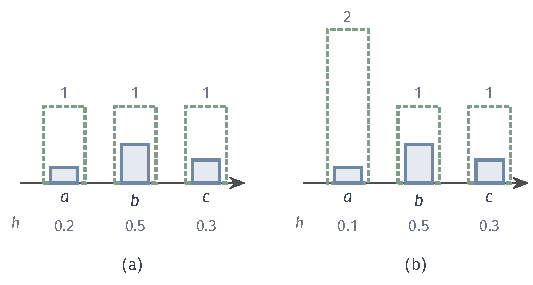
\includegraphics[width=90.255mm]{figures/04-spaces-measures-and-geometry/02-measure/tikz/dens-mass-ratio/figure.pdf}
  \caption{密度是目标质量与参考质量之比。三点集$\{a,b,c\}$上的目标质量$(0.2,0.5,0.3)$（蓝色实心柱）保持不变。(a)参考为计数测度（绿色虚线框高为$1$），每点的密度$h$等于目标质量本身；(b)参考权重改为$(2,1,1)$，点$a$的密度变为$0.2/2=0.1$，其余两点不变。}
  \label{fig:dens-mass-ratio}
\end{BookInlineFigure}

在实轴的长度测度下，每个单点的长度都是$0$，“单点质量相除”变成$0/0$，一般情形不能逐点定义比值，对角矩阵的类比在这里失效。可以保留的是另一半：在每个集合上，参考质量乘以权重再累计，应当得到目标质量。在有限点集上累计是求和，一般情形下就是第~\ref{chap:integration}章的积分。下面约定
\[
\int_Ah\,\mathrm d\mu=\int_Xh\mathbf 1_A\,\mathrm d\mu .
\]

\paragraph{加权测度}
先说明“给定权重，产生测度”总是可行的。这一方向相当于用对角矩阵去乘向量，不需要任何条件。

\begin{theorem}[加权测度]
\label{thm:dens-weighted-measure}
设$(X,\mathcal A,\mu)$是测度空间，$h:X\to[0,+\infty]$可测。令
\begin{equation}
\nu_h(A)=\int_Ah\,\mathrm d\mu ,\qquad A\in\mathcal A .
\label{eq:dens-weighted}
\end{equation}
则$\nu_h$是$(X,\mathcal A)$上的非负测度，并且$\nu_h\ll\mu$。
\end{theorem}

\begin{proof}
空集上的被积函数恒为零，所以$\nu_h(\varnothing)=0$，且$\nu_h$取值于$[0,+\infty]$。

设$A_1,A_2,\ldots\in\mathcal A$两两不交，$A=\bigcup_nA_n$。各$A_n$不交，所以逐点有
\[
h\mathbf 1_A=\sum_{n\geq1}h\mathbf 1_{A_n} .
\]
部分和是递增的非负可测函数列，由单调收敛定理可以逐项积分，得到
\[
\nu_h(A)=\int_Xh\mathbf 1_A\,\mathrm d\mu=\sum_{n=1}^\infty\int_Xh\mathbf 1_{A_n}\,\mathrm d\mu=\sum_{n=1}^\infty\nu_h(A_n).
\]
所以$\nu_h$可数可加。

若$\mu(A)=0$，函数$h\mathbf 1_A$在$\mu$零测集之外为零，其积分为$0$，故$\nu_h(A)=0$，即$\nu_h\ll\mu$。
\end{proof}

证明只用了单调收敛定理，没有要求$\mu$或$h$有限。若$h$在一个正测度集合上取$+\infty$，$\nu_h$可能连$\sigma$有限都不是，但它仍是测度。定理的最后一句说明：凡是能由参考测度加权得到的测度，都相对于参考测度绝对连续。

\begin{definition}[相对密度]
\label{def:dens-relative-density}
设$\mu,\nu$是$(X,\mathcal A)$上的非负测度。若可测函数$h:X\to[0,+\infty]$满足
\begin{equation}
\nu(A)=\int_Ah\,\mathrm d\mu ,\qquad A\in\mathcal A ,
\label{eq:dens-definition}
\end{equation}
就称$h$是$\nu$相对于$\mu$的一个\term{相对密度}（relative density），也称\term{Radon–Nikodym密度}（Radon-Nikodym derivative），记作$\dfrac{\mathrm d\nu}{\mathrm d\mu}=h$；$\mu$称为\term{参考测度}（reference measure）。
\end{definition}

密度的数值同时依赖目标测度与参考测度：上面的三点例子中，同一个$\nu$换一个参考，点$a$的密度就从$0.2$变为$0.1$。记号$\mathrm d\nu/\mathrm d\mu$借用了导数的写法，但它不是对某个坐标求导，而是两种测度之间的换算权重。由定理~\ref{thm:dens-weighted-measure}，密度存在的一个必要条件是$\nu\ll\mu$。

\paragraph{几乎处处版本}
定义说的是“一个”密度。若$h=g$在$\mu$几乎处处成立，则对每个$A$，$h\mathbf 1_A$与$g\mathbf 1_A$也$\mu$几乎处处相等，积分相同，所以$h,g$生成同一个测度。在$[0,1]$上，$h=1$与$g=1+\mathbf 1_{\mathbb Q\cap[0,1]}$都给出$\lambda|_{[0,1]}$，因为二者只在可数集上不同。

因此记号$\mathrm d\nu/\mathrm d\mu$只指其中任一个版本，关于密度的逐点断言，如“$h>0$”“$h<\infty$”，都只在$\mu$几乎处处的意义下才有意义。这与有限点集上不同：在每点都有正质量时，比值逐点确定；在长度下，单点不承载质量，所以单点上的值不算数。

\begin{example}[分段常值密度]
\label{ex:dens-piecewise}
在$[0,1]$上取$\mu=\lambda|_{[0,1]}$，并令
\[
h=\tfrac32\mathbf 1_{[0,1/2)}+\tfrac12\mathbf 1_{[1/2,1]} .
\]
由简单函数的积分，在每一块上把参考质量乘以该块的系数再相加：
\[
\nu_h(E)=\tfrac32\lambda\bigl(E\cap[0,\tfrac12)\bigr)+\tfrac12\lambda\bigl(E\cap[\tfrac12,1]\bigr).
\]
取$E=[0,1]$，得到
\[
\nu_h([0,1])=\tfrac32\cdot\tfrac12+\tfrac12\cdot\tfrac12=\tfrac34+\tfrac14=1 ,
\]
所以$\nu_h$是概率测度。对$E=[1/4,3/4]$，两块的长度各为$\tfrac14$，于是
\[
\nu_h(E)=\tfrac32\cdot\tfrac14+\tfrac12\cdot\tfrac14=\tfrac38+\tfrac18=\tfrac12 .
\]
\end{example}

图~\ref{fig:dens-weighted-measure}(a)中，$E$的质量$\tfrac12$就是$E$上方、密度图像之下的面积。(b)说明在零测点上改动密度不改变面积，这是“几乎处处版本”的几何含义。

\begin{BookInlineFigure}
  \centering
  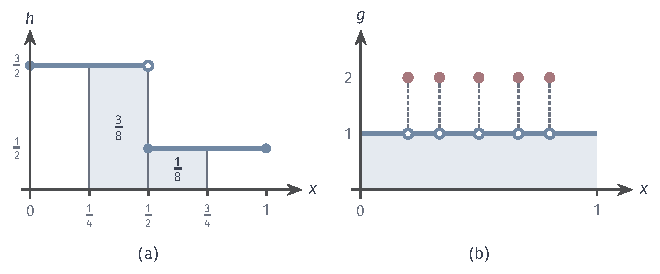
\includegraphics[width=111.693mm]{figures/04-spaces-measures-and-geometry/02-measure/tikz/dens-weighted-measure/figure.pdf}
  \caption{由密度构造测度，以及几乎处处版本。(a)参考测度为$[0,1]$上的长度，密度$h$在$[0,1/2)$上取$3/2$、在$[1/2,1]$上取$1/2$；集合$A=[1/4,3/4]$的质量$\nu_h(A)$是$A$上方的阴影面积$3/8+1/8=1/2$。(b)常数密度$1$与在若干零测点（红点，示意有理点）上改取$2$的函数$g$给出同一测度，因为改动的位置不承载长度。}
  \label{fig:dens-weighted-measure}
\end{BookInlineFigure}

概率论中的概率质量函数与概率密度函数都是这一定义的特例，区别只在参考测度：前者相对于可数集上的计数测度，后者相对于Lebesgue测度，可参考\BookChapterRef{chap:random-variables}{卷七第2章“随机变量的分布”}。一般的密度不要求总积分为一，$\int_Xh\,\mathrm d\mu=\nu(X)$只在目标是概率测度时等于$1$。

概率密度在某点的值也可以大于$1$，上例中$h$在$[0,1/2)$上就等于$\tfrac32$。密度值不是该点的概率，只有在集合上积分后才成为质量。

\subsection{Radon–Nikodym定理}
\label{sec:dens-radon-nikodym}

现在反过来：给定两个测度，能否找到同一个函数$h$，使式~\eqref{eq:dens-definition}对所有可测集同时成立？$\nu\ll\mu$是必要条件。它是否充分是一个真正的问题，因为要同时满足的等式有不可数多个，而绝对连续只告诉我们零测集的信息。

在有限点集上答案是直接的：$\nu\ll\mu$表示$m_i=0$时$p_i=0$，所以在$m_i>0$处令$h_i=p_i/m_i$，在$m_i=0$处任取一个值，就得到密度。一般情形没有逐点比值可用，下面的定理用一种优化的办法把比值“求”出来。

\begin{theorem}[Radon–Nikodym定理]
\label{thm:dens-radon-nikodym}
设$\mu,\nu$是$(X,\mathcal A)$上的$\sigma$有限非负测度，且$\nu\ll\mu$。则存在可测函数$h:X\to[0,+\infty)$，使
\begin{equation}
\nu(A)=\int_Ah\,\mathrm d\mu ,\qquad A\in\mathcal A .
\label{eq:dens-rn}
\end{equation}
若可测函数$g:X\to[0,+\infty]$也满足这一等式，则$g=h$在$\mu$几乎处处成立。
\end{theorem}

把\term{Radon–Nikodym定理}（Radon-Nikodym theorem）与定理~\ref{thm:dens-weighted-measure}对照：那里从$h$得到测度，这里从测度得到$h$。在$\sigma$有限范围内，“$\nu$相对于$\mu$有密度”与“$\nu\ll\mu$”是同一件事。证明先处理两个测度都有限的情形，再用$\sigma$有限性把空间切成可数个有限块。

\paragraph{有限情形：取最大的候选权重}
思路是在所有“处处不超过$\nu$”的权重中找一个积分最大的。把权重想成一层一层往上堆的沙子：每个集合上堆出的量都不能超过$\nu$在该集合上的质量。若某个权重已经堆到不能再高，那么它在每个集合上就应该恰好等于$\nu$。

\begin{lemma}[有限测度的密度存在]
\label{lem:dens-rn-finite}
设$\mu,\nu$是$(X,\mathcal A)$上的有限非负测度，且$\nu\ll\mu$。则存在可测函数$h:X\to[0,+\infty)$，使
\begin{equation}
\nu(A)=\int_Ah\,\mathrm d\mu ,\qquad A\in\mathcal A .
\label{eq:dens-rn-finite}
\end{equation}
\end{lemma}

\begin{proof}
第一步，证明候选权重对取最大值封闭。令
\[
\mathcal G=\Bigl\{g:X\to[0,+\infty]\text{可测}:\ \int_Ag\,\mathrm d\mu\leq\nu(A)\ \ \forall A\in\mathcal A\Bigr\}.
\]
零函数属于$\mathcal G$。设$g_1,g_2\in\mathcal G$，$g=\max(g_1,g_2)$。对任意$A$，令
\[
A_1=A\cap\{g_1\geq g_2\},\qquad A_2=A\cap\{g_1<g_2\}.
\]
二者可测、不交且并为$A$，于是
\[
\begin{aligned}
\int_Ag\,\mathrm d\mu&=\int_{A_1}g_1\,\mathrm d\mu+\int_{A_2}g_2\,\mathrm d\mu\\
&\leq\nu(A_1)+\nu(A_2)=\nu(A),
\end{aligned}
\]
故$g\in\mathcal G$。归纳可知有限个候选的最大值仍是候选。

第二步，用单调序列达到上确界。令
\[
s=\sup_{g\in\mathcal G}\int_Xg\,\mathrm d\mu\leq\nu(X)<\infty .
\]
取$g_n\in\mathcal G$使$\int_Xg_n\,\mathrm d\mu\to s$，再令$h_n=\max(g_1,\ldots,g_n)\in\mathcal G$。$h_n$递增，且
\[
\int_Xg_n\,\mathrm d\mu\leq\int_Xh_n\,\mathrm d\mu\leq s .
\]
令$h=\lim_nh_n$。由单调收敛定理，对每个$A$，
\[
\int_Ah\,\mathrm d\mu=\lim_{n\to\infty}\int_Ah_n\,\mathrm d\mu\leq\nu(A),
\]
所以$h\in\mathcal G$，并且$\int_Xh\,\mathrm d\mu=s$。由于这个积分有限，$h$只在$\mu$零测集上取$+\infty$，把这些值改为$0$不改变任何积分，所以可设$h$处处有限。

第三步，证明剩余质量为零。令
\[
r(A)=\nu(A)-\int_Ah\,\mathrm d\mu\geq0 .
\]
$\nu$与$\nu_h$都是有限测度，逐项相减可知$r$是有限非负测度。又$r\leq\nu$，所以$r\ll\mu$。

反设$r(X)>0$，则由$r\ll\mu$得$\mu(X)>0$。取
\[
\varepsilon=\frac{r(X)}{2\mu(X)} ,\qquad\text{于是}\quad(r-\varepsilon\mu)(X)=\frac{r(X)}2>0 .
\]
$r-\varepsilon\mu$是两个有限测度之差，是有限有符号测度。由第~\ref{chap:measure}章的Hahn分解，存在可测集$P$，使$P$的每个可测子集上$r-\varepsilon\mu\geq0$，$X\setminus P$的每个可测子集上$r-\varepsilon\mu\leq0$。

先说明$\mu(P)>0$。因为$(r-\varepsilon\mu)(X\setminus P)\leq0$，所以
\[
(r-\varepsilon\mu)(P)\geq(r-\varepsilon\mu)(X)>0 ,
\]
从而$r(P)>0$，再由$r\ll\mu$得$\mu(P)>0$。

再说明$h+\varepsilon\mathbf 1_P$仍是候选。对任意$A$，子集$A\cap P$上$r-\varepsilon\mu\geq0$，所以
\[
\varepsilon\mu(A\cap P)\leq r(A\cap P)\leq r(A).
\]
代回候选的积分，得到
\[
\begin{aligned}
\int_A(h+\varepsilon\mathbf 1_P)\,\mathrm d\mu
&=\int_Ah\,\mathrm d\mu+\varepsilon\mu(A\cap P)\\
&\leq\int_Ah\,\mathrm d\mu+r(A)=\nu(A).
\end{aligned}
\]
但它的总积分为$s+\varepsilon\mu(P)>s$，与$s$是上确界矛盾。因此$r(X)=0$，$r$在每个集合上为零，这就是式~\eqref{eq:dens-rn-finite}。
\end{proof}

第三步说明了为什么最大候选不留剩余：只要剩余质量$r$不为零，Hahn分解就能找到一块正测度区域，在那里$r$至少是参考测度的$\varepsilon$倍，于是可以把权重再加高$\varepsilon$。下面用一个两点的例子，把这一步的每个数都算出来。

\begin{example}[剩余质量怎样把候选抬高]
\label{ex:dens-rn-step}
取$X=\{a,b\}$，$\mu=\delta_a+2\delta_b$，$\nu=3\delta_a+\delta_b$。候选权重$g$只有两个数$g_a,g_b$，它在单点上的条件是
\[
g_a\cdot1\leq3,\qquad g_b\cdot2\leq1 .
\]
于是积分最大的候选是$(3,\tfrac12)$，它恰好就是质量之比，并且$s=3+1=4=\nu(X)$。

假设手里的候选还没到最大，取$h=(2,\tfrac12)$，它的总积分是$2+1=3<4$。剩余质量是
\[
r=\nu-h\mu=(3,1)-(2,1)=(1,0),\qquad r(X)=1 .
\]
证明中的$\varepsilon$取为
\[
\varepsilon=\frac{r(X)}{2\mu(X)}=\frac1{2\cdot3}=\frac16 .
\]
于是$r-\varepsilon\mu$在两点的值为
\[
1-\tfrac16\cdot1=\tfrac56,\qquad0-\tfrac16\cdot2=-\tfrac13 ,
\]
两数相加正好是$r(X)/2=\tfrac12$。Hahn分解的正集是$P=\{a\}$。

把$h$在$P$上加高$\varepsilon$，得到$h'=(\tfrac{13}6,\tfrac12)$。它在两点产生的质量是
\[
\tfrac{13}6\cdot1=\tfrac{13}6\leq3,\qquad\tfrac12\cdot2=1\leq1 ,
\]
仍是候选，而总积分从$3$升到$\tfrac{13}6+1=\tfrac{19}6$。只要$r$不为零，这样的抬高总能进行，所以最大的候选不留剩余。
\end{example}

图~\ref{fig:dens-rn-candidate}用连续的例子示意同一步。图中的$f$在证明中事先未知，这里画出只为便于观察；重要的是绿色条带仍在$f$之下，所以抬高后的函数仍是候选。

\begin{BookInlineFigure}
  \centering
  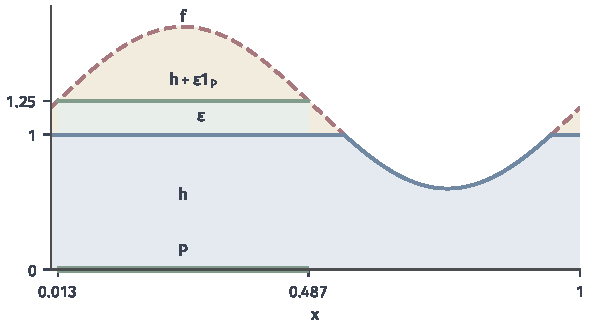
\includegraphics[width=100mm]{figures/04-spaces-measures-and-geometry/02-measure/matplotlib/dens-rn-candidate/figure.pdf}
  \caption{有限情形证明第三步的示意。参考测度为$[0,1]$上的长度，目标测度的密度$f(x)=1.2+0.6\sin(2\pi x)$（红色虚线）。候选$h=\min(f,1)$（蓝色实线）之下的质量已被表示，$h$与$f$之间的黄色区域是剩余质量$r$。取$\varepsilon=0.25$，正集$P=\{f-h\geq\varepsilon\}$约为$[0.013,0.487]$；在$P$上加高$\varepsilon$的绿色条带仍在$f$之下，所以$h+\varepsilon\mathbf 1_P$仍是候选而总积分更大。}
  \label{fig:dens-rn-candidate}
\end{BookInlineFigure}

\begin{proof}[定理~\ref{thm:dens-radon-nikodym}的证明]
先作有限分块。由$\sigma$有限性，存在两两不交的可测集$A_i$覆盖$X$且$\mu(A_i)<\infty$，以及两两不交的可测集$B_j$覆盖$X$且$\nu(B_j)<\infty$。可数族$\{A_i\cap B_j\}$两两不交、覆盖$X$，每块上$\mu,\nu$都有限，把它们排成一列$X_1,X_2,\ldots$。

再证存在性。对每个$k$，令
\[
\mu_k(A)=\mu(A\cap X_k),\qquad\nu_k(A)=\nu(A\cap X_k).
\]
这是两个有限测度，且$\nu_k\ll\mu_k$。由引理~\ref{lem:dens-rn-finite}，存在有限值可测函数$h_k$，使
\[
\nu(A\cap X_k)=\int_Ah_k\,\mathrm d\mu_k=\int_Ah_k\mathbf 1_{X_k}\,\mathrm d\mu ,
\]
后一个等号先对指示函数核对，再经简单函数与单调收敛推广。

令$h=\sum_kh_k\mathbf 1_{X_k}$，各$X_k$不交，每点至多一项非零，$h$有限且可测。由$\nu$的可数可加性与非负级数的逐项积分，
\[
\nu(A)=\sum_k\nu(A\cap X_k)=\sum_k\int_Ah_k\mathbf 1_{X_k}\,\mathrm d\mu=\int_Ah\,\mathrm d\mu .
\]

最后证唯一性。设$g:X\to[0,+\infty]$也满足等式。固定$k$，令$D=X_k\cap\{h>g\}$，则
\[
\int_Dh\,\mathrm d\mu=\nu(D)=\int_Dg\,\mathrm d\mu ,
\]
两边不超过$\nu(X_k)<\infty$，于是$\int_D(h-g)\,\mathrm d\mu=0$。被积函数在$D$上严格为正，所以$\mu(D)=0$。同理$\mu(X_k\cap\{g>h\})=0$。对$k$取可数并，$\{g\neq h\}$是$\mu$零测集。
\end{proof}

唯一性证明中只有一处用到有限性：$\nu(X_k)<\infty$才能把两个相等的积分相减。这里实际只需要$\nu$是$\sigma$有限的。缺少这一条件时唯一性可以失败：单点空间$X=\{0\}$上取$\mu(\{0\})=+\infty$，$\nu=\mu$，常数$1$与常数$2$都满足
\[
\int_{\{0\}}h\,\mathrm d\mu=+\infty=\nu(\{0\}),
\]
却在一个$\mu$测度为$+\infty$的集合上不同。所以密度只在$\mu$几乎处处的意义下唯一，而且这一唯一性依赖目标测度的$\sigma$有限性。

\paragraph{有限性条件不能随意去掉}
存在性同样依赖参考测度的$\sigma$有限性。在$[0,1]$的Borel集上取计数测度$c$与Lebesgue测度$\lambda$。$c(A)=0$只在$A=\varnothing$时成立，所以$\lambda\ll c$。若存在可测$h\geq0$使$\lambda(A)=\int_Ah\,\mathrm dc$，取$A=\{x\}$，就得到
\[
0=\lambda(\{x\})=h(x)c(\{x\})=h(x).
\]
于是$h$处处为零，却要给出$\lambda([0,1])=1$，矛盾。失效的原因在于$c$的有限测度集只能是有限集，可数个有限集之并盖不住$[0,1]$，$c$不是$\sigma$有限的。

这个反例说明定理不能无条件推广，但不说明$\sigma$有限是密度存在的必要条件。仍以$c$为参考，$\delta_0$有密度$\mathbf 1_{\{0\}}$，因为
\[
\int_A\mathbf 1_{\{0\}}\,\mathrm dc=c(A\cap\{0\})=\delta_0(A).
\]
$\sigma$有限是本章采用的一组充分条件。

\paragraph{有限有符号测度的密度}
第~\ref{chap:measure}章的有限有符号测度允许集合质量为负，它由Jordan分解写成两个有限测度之差$\eta=\eta^+-\eta^-$，总变差为$\lvert\eta\rvert=\eta^++\eta^-$。不能把上面的定理直接套到任意两个测度之差上：两个无限测度之差可能在某些集合上是$\infty-\infty$，根本没有定义。对有限有符号测度，可以对两个变差分别求密度。

\begin{theorem}[有限有符号测度的密度]
\label{thm:dens-signed}
设$\mu$是$(X,\mathcal A)$上的$\sigma$有限非负测度，$\eta$是有限有符号测度。则$\lvert\eta\rvert\ll\mu$当且仅当存在$\mu$可积的实值函数$h$，使
\begin{equation}
\eta(A)=\int_Ah\,\mathrm d\mu ,\qquad A\in\mathcal A .
\label{eq:dens-signed}
\end{equation}
此时$h$在$\mu$几乎处处意义下唯一，并且对每个$A\in\mathcal A$，
\begin{equation}
\eta^\pm(A)=\int_Ah^\pm\,\mathrm d\mu,\qquad\lvert\eta\rvert(A)=\int_A\lvert h\rvert\,\mathrm d\mu ,
\label{eq:dens-signed-parts}
\end{equation}
其中$h^+=\max(h,0)$，$h^-=\max(-h,0)$。
\end{theorem}

\begin{proof}
设$\lvert\eta\rvert\ll\mu$。由$\eta^\pm\leq\lvert\eta\rvert$得$\eta^\pm\ll\mu$。$\eta^\pm$是有限测度，由定理~\ref{thm:dens-radon-nikodym}得到有限值密度$h_1,h_2$，并且
\[
\int_Xh_1\,\mathrm d\mu=\eta^+(X)<\infty,\qquad\int_Xh_2\,\mathrm d\mu=\eta^-(X)<\infty ,
\]
二者都可积。令$h=h_1-h_2$，由可积函数积分的线性性，$h$满足式~\eqref{eq:dens-signed}。

反过来，设式~\eqref{eq:dens-signed}成立且$h$可积。令$P=\{h\geq0\}$。$P$的每个可测子集上$\eta\geq0$，补集的每个可测子集上$\eta\leq0$，所以$P$与$X\setminus P$构成$\eta$的一组Hahn分解。由Jordan分解，
\[
\eta^+(A)=\eta(A\cap P)=\int_Ah^+\,\mathrm d\mu ,
\]
\[
\eta^-(A)=-\eta(A\setminus P)=\int_Ah^-\,\mathrm d\mu .
\]
两式相加就得到$\lvert\eta\rvert$的表示，这就是式~\eqref{eq:dens-signed-parts}。由定理~\ref{thm:dens-weighted-measure}，$\lvert\eta\rvert\ll\mu$。

这一段对前一段构造的$h$同样适用，所以式~\eqref{eq:dens-signed-parts}在两个方向上都成立。

唯一性方面，若可积的$h,h'$都满足式~\eqref{eq:dens-signed}，令$D=\{h>h'\}$，则两个有限积分相等，得到
\[
\int_D(h-h')\,\mathrm d\mu=0 .
\]
被积函数在$D$上严格为正，所以$\mu(D)=0$。交换$h,h'$得$\mu(\{h'>h\})=0$，于是$h=h'$在$\mu$几乎处处成立。
\end{proof}

定理把集合层面的正负分解翻译成函数层面的正负部：Hahn分解的正区域可以取为$\{h\geq0\}$，Jordan分解的两项就是$h^+$与$h^-$分别生成的测度。可积性在这里是自然的，因为由式~\eqref{eq:dens-signed-parts}，$\lvert h\rvert$的积分就是有限的总变差$\lvert\eta\rvert(X)$。

例如$[0,1]$上$h(x)=1-2x$生成的$\eta$，正集是$P=[0,\tfrac12]$，两个变差的总质量都可以算出：
\[
\eta^+([0,1])=\int_0^{1/2}(1-2x)\,\mathrm dx=\tfrac14,\qquad\eta^-([0,1])=\int_{1/2}^1(2x-1)\,\mathrm dx=\tfrac14 .
\]
所以$\eta([0,1])=0$，正负质量完全抵消，而$\lvert\eta\rvert([0,1])=\tfrac12$记录了被抵消掉的变化总量。

\section{测度的分解}
\label{sec:dens-decomposition}

绝对连续与相互奇异是两个极端：前者不在参考测度的零测集上放任何质量，后者把全部质量放在某个参考零测集上。一般的测度介于两者之间，例如长度加上一个点质量。本节先证明，相对于给定的参考测度，$\sigma$有限测度都能唯一地拆成这两种极端之和，并用Radon–Nikodym定理表示其中绝对连续的一份。然后在实轴上以Lebesgue测度为参考，把奇异的一份再分成点质量与没有点质量的奇异质量，并说明累积函数的普通导数只能读出其中哪一部分。

\subsection{Lebesgue分解}
\label{sec:dens-lebesgue-decomposition}

给定参考测度$\mu$与目标测度$\nu$，我们希望把$\nu$的质量分成两份：一份完全落在某个$\mu$零测集上，是$\mu$“看不见”的质量；另一份在$\mu$零测集上没有任何质量。分解有三个问题需要分别回答：两份质量怎样构造，分法是否唯一，以及看得见的那份能否写成密度。

\begin{theorem}[Lebesgue分解]
\label{thm:dens-lebesgue-decomposition}
设$\mu,\nu$是可测空间$(X,\mathcal A)$上的$\sigma$有限非负测度。则存在唯一的一对非负测度$\nu_{\mathrm{ac}},\nu_{\mathrm s}$，使
\[
\nu=\nu_{\mathrm{ac}}+\nu_{\mathrm s},\qquad\nu_{\mathrm{ac}}\ll\mu,\qquad\nu_{\mathrm s}\perp\mu .
\]
更具体地，存在$N\in\mathcal A$使$\mu(N)=0$，$\nu_{\mathrm s}(A)=\nu(A\cap N)$，$\nu_{\mathrm{ac}}(A)=\nu(A\setminus N)$。并且存在可测函数$h:X\to[0,+\infty)$，使
\begin{equation}
\nu(A)=\int_Ah\,\mathrm d\mu+\nu_{\mathrm s}(A),\qquad A\in\mathcal A ,
\label{eq:dens-lebesgue-form}
\end{equation}
$h$在$\mu$几乎处处意义下唯一。特别地，$\nu$相对于$\mu$有密度，当且仅当$\nu_{\mathrm s}=0$。
\end{theorem}

这一分解称为$\nu$相对于$\mu$的\term{Lebesgue分解}（Lebesgue decomposition），$\nu_{\mathrm{ac}}$与$\nu_{\mathrm s}$分别称为绝对连续部分与奇异部分。分解依赖参考测度。在实轴上取$\nu=\lambda|_{[0,1]}+\delta_2$。以$\lambda$为参考，$N=\{2\}$是$\lambda$零测集并承载点质量，于是$\nu_{\mathrm s}=\delta_2$，$\nu_{\mathrm{ac}}=\lambda|_{[0,1]}$。以$\delta_2$为参考，$\mathbb R\setminus\{2\}$是$\delta_2$零测集，角色互换：$\nu_{\mathrm s}=\lambda|_{[0,1]}$，$\nu_{\mathrm{ac}}=\delta_2$。

\paragraph{构造：承载最多质量的零测集}
定理中的$N$应当在保持$\mu(N)=0$的同时尽可能多地装下$\nu$的质量。若某个$\mu$零测集在$N$之外还有正的$\nu$质量，就把它并进$N$。先在$\nu$有限时用上确界实现这个想法。

\begin{proof}[存在性，$\nu$有限的情形]
令$M=\sup\{\nu(A):A\in\mathcal A,\ \mu(A)=0\}\leq\nu(X)<\infty$。对每个$k$取$\mu$零测集$N_k$使$\nu(N_k)>M-1/k$，令$N=\bigcup_kN_k$。由可数次可加性$\mu(N)=0$，所以$\nu(N)\leq M$；又$\nu(N)\geq\nu(N_k)>M-1/k$，故$\nu(N)=M$。

令$\nu_{\mathrm s}(A)=\nu(A\cap N)$，$\nu_{\mathrm{ac}}(A)=\nu(A\setminus N)$，二者都是测度，和为$\nu$。由$\mu(N)=0$与$\nu_{\mathrm s}(X\setminus N)=0$得$\nu_{\mathrm s}\perp\mu$。设$\mu(A)=0$，则$N\cup(A\setminus N)$仍是$\mu$零测集，其$\nu$质量不超过$M$；两部分不交，所以$M+\nu(A\setminus N)\leq M$。$M$有限，消去得$\nu_{\mathrm{ac}}(A)=0$，即$\nu_{\mathrm{ac}}\ll\mu$。
\end{proof}

最后的消去正是需要有限性的地方：若$M=+\infty$，不等式$M+t\leq M$不能推出$t=0$。对$\sigma$有限的$\nu$，取两两不交的$X_j$覆盖$X$且$\nu(X_j)<\infty$，在每片上对有限测度$A\mapsto\nu(A\cap X_j)$作上面的构造，得到$\mu$零测集$N_j\subset X_j$；令$N=\bigcup_jN_j$，则$\mu(N)=0$。若$\mu(A)=0$，则$\nu(A\setminus N)=\sum_j\nu((A\setminus N_j)\cap X_j)=0$，每一项是相应片上已证的绝对连续性。构造只用了可数次可加性、上确界与限制测度，没有用积分。

\paragraph{唯一性}
设$\nu=\alpha+\beta=\alpha'+\beta'$，其中$\alpha,\alpha'\ll\mu$，$\beta,\beta'\perp\mu$。取$\mu$零测集$S,S'$使$\beta(X\setminus S)=0$，$\beta'(X\setminus S')=0$，令$T=S\cup S'$，则$\mu(T)=0$，$\beta,\beta'$在$X\setminus T$上都没有质量。对任意$A$，$\mu(A\cap T)=0$推出$\alpha(A\cap T)=\alpha'(A\cap T)=0$，所以$\beta(A\cap T)=\nu(A\cap T)=\beta'(A\cap T)$；又$\beta(A\setminus T)=\beta'(A\setminus T)=0$，所以$\alpha(A\setminus T)=\nu(A\setminus T)=\alpha'(A\setminus T)$。两部分相加，得$\alpha=\alpha'$，$\beta=\beta'$。

唯一性的论证只在$T$与$X\setminus T$上分别读取$\nu$，没有做减法，因此不需要任何有限性。$\sigma$有限条件只在存在性中用到，并且不能随意去掉：在$[0,1]$的Borel集上取$\mu=\lambda$，$\nu$为计数测度。若有满足要求的分解，取$N$使$\lambda(N)=0$、$\nu_{\mathrm s}([0,1]\setminus N)=0$；由于$\lambda(N)=0$，可取$x\notin N$，则$\nu_{\mathrm s}(\{x\})=0$，而$\lambda(\{x\})=0$又给出$\nu_{\mathrm{ac}}(\{x\})=0$，于是$\nu(\{x\})=0$，与计数测度矛盾。

\paragraph{密度表示}
最后一步才用到Radon–Nikodym定理。$\nu_{\mathrm{ac}}\leq\nu$，所以盖住$X$的$\nu$有限块也使$\nu_{\mathrm{ac}}$有限，$\nu_{\mathrm{ac}}$是$\sigma$有限的；对$\nu_{\mathrm{ac}}\ll\mu$应用定理~\ref{thm:dens-radon-nikodym}，得到$h=\mathrm d\nu_{\mathrm{ac}}/\mathrm d\mu$，这就是式~\eqref{eq:dens-lebesgue-form}。若另有$(h',\nu_{\mathrm s}')$满足同样的表示，则$A\mapsto\int_Ah'\,\mathrm d\mu$绝对连续（定理~\ref{thm:dens-weighted-measure}），由分解的唯一性它等于$\nu_{\mathrm{ac}}$，再由Radon–Nikodym定理的唯一性得$h'=h$几乎处处。若$\nu$有密度，则$\nu\ll\mu$，$\nu=\nu+0$就是它的分解，所以$\nu_{\mathrm s}=0$；反之$\nu_{\mathrm s}=0$时$h$就是$\nu$的密度。

三部分的依据各不相同：构造依靠可数次可加性与上确界，唯一性只读取两个集合上的值，密度表示则依靠Radon–Nikodym定理。奇异部分无论如何写不成相对于$\mu$的密度，因为它集中在一个$\mu$零测集上，而任何密度在零测集上的积分都是$0$。若目标是有限有符号测度，可以对第~\ref{chap:measure}章Jordan分解的两个变差分别作Lebesgue分解；正负分解本身回用那里的结论，这里不再重复。

\subsection{实轴测度的分解}
\label{sec:dens-real-line-decomposition}

在实轴上以$\lambda$为参考时，单点都是$\lambda$零测集，所以点质量一定属于奇异部分。问题是奇异部分是否只有点质量。下面先以实轴上的有限Borel测度为对象，把点质量完整地提出来，再说明余下的奇异部分可以不为零。

\paragraph{原子至多可数}
设$\rho$是$\mathcal B(\mathbb R)$上的有限测度。若$\rho(\{x\})>0$，称$x$是$\rho$的一个\term{原子}（atom）。

\begin{lemma}[原子至多可数]
\label{lem:dens-atoms-countable}
有限Borel测度$\rho$的原子集$D=\{x\in\mathbb R:\rho(\{x\})>0\}$至多可数。
\end{lemma}

\begin{proof}
令$D_k=\{x:\rho(\{x\})>1/k\}$，则$D=\bigcup_kD_k$。若$x_1,\ldots,x_m$是$D_k$中互不相同的点，有限可加性给出$m/k<\sum_{i=1}^m\rho(\{x_i\})\leq\rho(\mathbb R)$，所以$D_k$至多有$k\rho(\mathbb R)$个点。可数个有限集之并至多可数。
\end{proof}

于是可以定义$\rho_{\mathrm d}(B)=\rho(B\cap D)=\sum_{x\in B\cap D}\rho(\{x\})$，它是全部点质量之和，称为$\rho$的离散部分；余下的$\rho_{\mathrm c}(B)=\rho(B\setminus D)$没有原子。

\begin{theorem}[实轴上有限测度的分解]
\label{thm:dens-three-part}
设$\rho$是$\mathcal B(\mathbb R)$上的有限测度。则$\rho$可以唯一地写成
\[
\rho=\rho_{\mathrm d}+\rho_{\mathrm{ac}}+\rho_{\mathrm{sc}},
\]
其中$\rho_{\mathrm d}$集中在一个至多可数集上，$\rho_{\mathrm{ac}}\ll\lambda$，$\rho_{\mathrm{sc}}\perp\lambda$且没有原子。没有原子且与$\lambda$相互奇异的测度称为\term{奇异连续测度}（singular continuous measure）。
\end{theorem}

\begin{proof}
存在性：对有限测度$\rho_{\mathrm c}$关于$\lambda$作Lebesgue分解，得$\rho_{\mathrm c}=\rho_{\mathrm{ac}}+\rho_{\mathrm{sc}}$，而$\rho_{\mathrm{sc}}(\{x\})\leq\rho_{\mathrm c}(\{x\})=0$。

唯一性：设$\rho=d+a+s$也满足条件，$d$集中在至多可数集$D'$上。$a\ll\lambda$给出$a(\{x\})=0$，$s$没有原子，所以$\rho(\{x\})=d(\{x\})$对每个$x$成立。于是$D\subset D'$，并且$d(B)=\sum_{x\in B\cap D'}d(\{x\})=\sum_{x\in B\cap D}\rho(\{x\})=\rho_{\mathrm d}(B)$，因为$D'\setminus D$中的点质量为零。由此$a+s=\rho-d=\rho_{\mathrm c}$（各项有限，减法有意义），再由Lebesgue分解的唯一性得$a=\rho_{\mathrm{ac}}$，$s=\rho_{\mathrm{sc}}$。
\end{proof}

离散部分集中在可数集上，与$\lambda$相互奇异，所以$\rho$相对于$\lambda$的奇异部分就是$\rho_{\mathrm d}+\rho_{\mathrm{sc}}$。三项是同一个测度的三个成分，一个测度可以同时含有三者，也可以缺少其中任意几项。

定理只对有限测度陈述。推广到$\sigma$有限的Borel测度时需要核对两点。其一，原子集仍至多可数：取测度有限且覆盖$\mathbb R$的可测集$X_1,X_2,\ldots$，每个原子落在某个$X_k$中，对有限测度$B\mapsto\rho(B\cap X_k)$用引理~\ref{lem:dens-atoms-countable}，可知$X_k$中的原子至多可数。其二，唯一性证明中的减法$\rho-d$可能出现$\infty-\infty$，应改为把各成分限制到每个$X_k$上分别比较。局部有限测度，即在每个有界区间上取有限值的测度，用$X_k=(k-1,k]$与$(-k,-k+1]$即可覆盖，是最常见的情形，例如Lebesgue测度本身。

\paragraph{累积函数读出原子}
离散部分可以从累积函数读出。记$G(x)=\rho((-\infty,x])$。集合$(-\infty,x-1/m]$递增到$(-\infty,x)$，由测度的从下连续性，左极限$G(x-)=\rho((-\infty,x))$，所以
\[
G(x)-G(x-)=\rho(\{x\}).
\]
$G$在$x$处跳跃当且仅当$x$是原子，$G$连续当且仅当$\rho_{\mathrm d}=0$。累积函数连续能排除离散部分，却不能排除奇异连续部分。下面的Cantor测度说明后者确实存在。

\paragraph{Cantor测度}
第~\ref{chap:integration}章构造了Cantor集$C\subset[0,1]$与Cantor函数$F_C$：$C$由逐步删去中间三分之一开区间得到，Lebesgue测度为零；$F_C$连续、单调不减，$F_C(0)=0$，$F_C(1)=1$，并在每个删去的开区间上为常数。把$F_C$延拓为$x<0$时取$0$、$x>1$时取$1$，延拓后的函数连续、单调不减，按第~\ref{chap:measure}章的Stieltjes构造得到Borel测度$\mu_C$，满足$\mu_C((a,b])=F_C(b)-F_C(a)$，称为\term{Cantor测度}（Cantor measure）。

它的三条性质可以直接核对。总质量为$F_C(1)-F_C(0)=1$。没有原子：$F_C$连续，所以$\mu_C(\{x\})=F_C(x)-F_C(x-)=0$。集中在$C$上：在每个删去的开区间$(a,b)$上$F_C$为常数，由从下连续性$\mu_C((a,b))=\lim_m(F_C(b-1/m)-F_C(a))=0$，两条半直线同理；$\mathbb R\setminus C$是这些开区间与两条半直线的可数并，故$\mu_C(\mathbb R\setminus C)=0$。又$\lambda(C)=0$，取$N=C$即得$\mu_C\perp\lambda$。所以$\mu_C$是一个非零的奇异连续测度。

\begin{example}[三种成分的混合]
\label{ex:dens-three-part-mixture}
令$\rho=\tfrac12\lambda|_{[0,1]}+\tfrac14\delta_{1/2}+\tfrac14\mu_C$，总质量$\tfrac12+\tfrac14+\tfrac14=1$。$\lambda$与$\mu_C$都没有原子，唯一的原子是$1/2$，所以$\rho_{\mathrm d}=\tfrac14\delta_{1/2}$。余下的$\tfrac12\lambda|_{[0,1]}+\tfrac14\mu_C$相对于$\lambda$作Lebesgue分解，取$N=C$：前一项在$C$上为零，后一项集中在$C$上，于是$\rho_{\mathrm{ac}}=\tfrac12\lambda|_{[0,1]}$，$\rho_{\mathrm{sc}}=\tfrac14\mu_C$。按式~\eqref{eq:dens-lebesgue-form}，$\rho$相对于$\lambda$的密度部分是$h=\tfrac12\mathbf 1_{[0,1]}$，图~\ref{fig:dens-lebesgue-form}画出了这三部分。
\end{example}

\begin{figure}[!htbp]
  \centering
  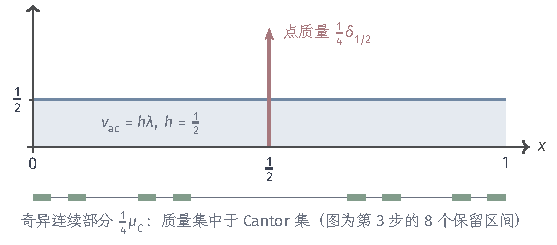
\includegraphics[width=94.365mm]{figures/02-abstract-mathematics/01-metric-and-measure/tikz/c4-lebesgue-density/figure.pdf}
  \caption{相对于长度测度的密度只表示绝对连续部分。$\rho=\tfrac12\lambda|_{[0,1]}+\tfrac14\delta_{1/2}+\tfrac14\mu_C$：蓝色区域是密度$h=1/2$表示的质量$1/2$；红色箭头是位于$1/2$的点质量$1/4$；下方绿色线段是Cantor集构造第$3$步保留的$8$个区间，Cantor测度的质量$1/4$集中在它们的极限——零长度的Cantor集上。后两部分都集中在长度零测集上，任何密度都无法表示。}
  \label{fig:dens-lebesgue-form}
\end{figure}

\paragraph{普通导数能恢复什么}
这个例子的累积函数在$[0,1]$上是$G(x)=\tfrac12x+\tfrac14\mathbf 1_{[1/2,\infty)}(x)+\tfrac14F_C(x)$。求它的普通导数：一次项的导数是$\tfrac12$；阶跃项在$x\neq1/2$处导数为零；Cantor函数在每个删去的开区间上为常数，而这些开区间的总长度为$1$，所以它几乎处处导数为零。于是$G'=\tfrac12$几乎处处，恰好是绝对连续部分的密度。

导数遗漏了另外两份质量：$\int_0^1G'\,\mathrm dx=\tfrac12$，而$G(1)-G(0)=1$，差额中$\tfrac14$是原点$1/2$处的跳跃，另$\tfrac14$是Cantor函数在零长度集合上的连续增长。这正是第~\ref{chap:integration}章所说的：连续性与几乎处处可导都不能保证函数由导数的积分恢复。一般地，实轴上有限Borel测度的累积函数几乎处处可导，导数几乎处处等于绝对连续部分的密度；这一结论属于Lebesgue微分定理，这里不给出证明。本章只在累积函数绝对连续时使用导数计算密度，见第~\ref{sec:dens-cumulative-density}小节。

\section{密度的运算}
\label{sec:dens-rules}

有了密度以后，最常用的操作都围绕“换参考测度”：把对目标测度的积分改写成对参考测度的加权积分；把几个目标测度相对同一参考的密度组合起来；经过一个中间测度连续换两次参考；或者把参考与目标的角色对调。本节在同一可测空间$(X,\mathcal A)$上依次建立这些规则，每条规则都注明所需的测度关系，以及等式在哪个测度的几乎处处意义下成立。

\subsection{换测度的积分公式}
\label{sec:dens-change-of-measure}

密度的定义~\eqref{eq:dens-definition}只说明指示函数$\mathbf 1_A$对$\nu$的积分等于$\mathbf 1_Ah$对$\mu$的积分。积分本来就是从指示函数出发，经简单函数和单调逼近推广到一般函数的，所以这个等式可以沿同一条路线推广。

\begin{theorem}[换测度公式]
\label{thm:dens-change-of-measure}
设$\mu,\nu$是$(X,\mathcal A)$上的非负测度，$h$是$\nu$相对于$\mu$的密度，约定$0\cdot(+\infty)=0$。
\begin{enumerate}
\item 对每个可测函数$f:X\to[0,+\infty]$，
\begin{equation}
\int_Xf\,\mathrm d\nu=\int_Xfh\,\mathrm d\mu .
\label{eq:dens-change-of-measure}
\end{equation}
\item 对实值或复值可测函数$f$，$f$对$\nu$可积当且仅当$fh$对$\mu$可积，此时式~\eqref{eq:dens-change-of-measure}成立。
\end{enumerate}
\end{theorem}

\begin{proof}
(1) 对$f=\mathbf 1_A$，两边分别是$\nu(A)$与$\int_Ah\,\mathrm d\mu$，由密度的定义相等。对非负简单函数，两边对$f$都是线性的，等式成立。对一般非负可测$f$，取非负简单函数列$s_n\uparrow f$。因$h\geq0$，$s_nh$也递增并逐点收敛到$fh$。两边分别用单调收敛定理，
\[
\int_Xf\,\mathrm d\nu=\lim_{n\to\infty}\int_Xs_n\,\mathrm d\nu=\lim_{n\to\infty}\int_Xs_nh\,\mathrm d\mu=\int_Xfh\,\mathrm d\mu ,
\]
两边允许同时为$+\infty$。

(2) 对$\lvert f\rvert$用(1)，得$\int\lvert f\rvert\,\mathrm d\nu=\int\lvert fh\rvert\,\mathrm d\mu$，两种可积性等价。实值时$(fh)^\pm=f^\pm h$，对$f^+,f^-$分别用(1)，各得两个有限数，相减即得等式。复值时对实部和虚部分别处理。
\end{proof}

\term{换测度公式}（change-of-measure formula）把“对目标测度累计”改写成“对参考测度加权累计”。被积的变量与函数$f$都不变，点不移动，改变的只是每一处的累计权重。例如$[0,1]$上$\nu$相对于长度的密度为$h(x)=2x$，取$f(x)=x$，则$\int f\,\mathrm d\nu=\int_0^1x\cdot2x\,\mathrm dx=\tfrac23$；若$\nu$是概率测度，这就是用概率密度计算期望的公式。

两部分的条件不同。非负函数不需要任何可积性，等式两边可以同为$+\infty$；实值或复值函数则必须先由$\lvert f\rvert$确认两边绝对可积，否则正部与负部的积分可能都是$+\infty$，不能相减。证明中没有用到$\mu,\nu$的有限性：只要密度存在，公式就成立。

\subsection{密度的线性组合}
\label{sec:dens-linear-combination}

相对同一个参考测度，几个目标测度组合起来时，密度怎样组合？非负组合可以直接相加；带符号的组合还要先保证测度之差有定义。

\paragraph{共同参考下的非负组合}
设$\nu_1,\ldots,\nu_m$相对于同一个参考测度$\mu$分别有密度$h_1,\ldots,h_m$，$a_1,\ldots,a_m\geq0$。由非负积分的线性性，对每个可测集$A$，
\[
\sum_{i=1}^ma_i\nu_i(A)=\sum_{i=1}^ma_i\int_Ah_i\,\mathrm d\mu=\int_A\sum_{i=1}^ma_ih_i\,\mathrm d\mu ,
\]
所以$\sum_ia_i\nu_i$的密度是$\sum_ia_ih_i$。关键是参考测度相同：密度是相对于参考的换算比例，只有同一种参考下的比例才能直接相加。非负系数的可数和同样成立，此时交换求和与积分的依据是单调收敛定理。

共同参考还能把一个相对于长度没有密度的测度写成单个函数的积分。

\begin{example}[点质量与长度的统一表示]
\label{ex:dens-mixed-reference}
在$[0,1]$上取参考测度$\mu=\lambda|_{[0,1]}+\delta_0$。对可测集$A\subset[0,1]$，
\begin{equation*}
\begin{aligned}
\int_A\mathbf 1_{(0,1]}\,\mathrm d\mu&=\lambda(A\cap(0,1])+\delta_0(A\cap(0,1])=\lambda(A),\\
\int_A\mathbf 1_{\{0\}}\,\mathrm d\mu&=\lambda(A\cap\{0\})+\delta_0(A\cap\{0\})=\delta_0(A),
\end{aligned}
\end{equation*}
其中用了$\lambda(\{0\})=0$与$0\notin(0,1]$。所以$\mathrm d\lambda|_{[0,1]}/\mathrm d\mu=\mathbf 1_{(0,1]}$，$\mathrm d\delta_0/\mathrm d\mu=\mathbf 1_{\{0\}}$。由线性组合规则，$a,b\geq0$时$\nu=a\lambda|_{[0,1]}+b\delta_0$的密度是$a\mathbf 1_{(0,1]}+b\mathbf 1_{\{0\}}$。当$b>0$时$\nu$在长度零测集$\{0\}$上有正质量，整体没有Lebesgue密度；换用共同参考$\mu$后，点质量与长度质量就由一个函数统一表示。
\end{example}

例中原点处的密度值$b$不能随意改动：原点在$\mu$下质量为$1$，不是$\mu$零测集。这与长度参考不同，那里单点上的取值可以任意改变。哪些点上的密度值有意义，取决于参考测度在那里有没有质量。

\paragraph{带符号的组合}
差需要谨慎处理。若$\nu_1,\nu_2$是有限测度，则$h_1,h_2$可积，$\eta=a\nu_1-b\nu_2$（$a,b$为实数）是有限有符号测度，由可积函数积分的线性性，它的密度是可积函数$ah_1-bh_2$，与定理~\ref{thm:dens-signed}一致。对无限测度不能这样做：在$\mathbb R$上取$\nu_1=\nu_2=\lambda$，形式上$h_1-h_2=0$，可$\nu_1(\mathbb R)-\nu_2(\mathbb R)=\infty-\infty$没有定义，“$\nu_1-\nu_2$”不是在所有集合上都有值的对象。更一般地，只要对相减的两项在所考虑的每个集合上都有$\int_Ah_2\,\mathrm d\mu<\infty$，差才有意义。


\subsection{链式规则}
\label{sec:dens-chain-rule}

换算比例可以连乘：先从一种参考换到中间测度，再从中间测度换到目标。为避免与Lebesgue测度的记号冲突，本小节用$\rho$表示最底层的参考测度。

\begin{theorem}[密度的链式规则]
\label{thm:dens-chain-rule}
设$\rho,\mu,\nu$是$(X,\mathcal A)$上的$\sigma$有限非负测度，且$\nu\ll\mu\ll\rho$。则$\nu\ll\rho$，并且
\[
\frac{\mathrm d\nu}{\mathrm d\rho}=\frac{\mathrm d\nu}{\mathrm d\mu}\cdot\frac{\mathrm d\mu}{\mathrm d\rho}\qquad\rho\text{几乎处处}.
\]
\end{theorem}

\begin{proof}
由Radon–Nikodym定理取$g=\mathrm d\nu/\mathrm d\mu$与$k=\mathrm d\mu/\mathrm d\rho$。对任意可测集$A$，先用$g$的定义，再对非负函数$\mathbf 1_Ag$与密度$k$使用换测度公式，
\[
\nu(A)=\int_X\mathbf 1_Ag\,\mathrm d\mu=\int_X\mathbf 1_Agk\,\mathrm d\rho .
\]
所以$gk$是$\nu$相对于$\rho$的一个密度，由定理~\ref{thm:dens-weighted-measure}得$\nu\ll\rho$。$\nu,\rho$都$\sigma$有限，由Radon–Nikodym定理的唯一性，任何版本的$\mathrm d\nu/\mathrm d\rho$都与$gk$在$\rho$几乎处处意义下相等。
\end{proof}

这条\term{密度的链式规则}（chain rule for densities）与一元微积分的链式法则形式相似，依据却是换测度公式，而不是对坐标求导。逐次换参考与直接换参考给出同一个积分表示：对非负$f$，$\int f\,\mathrm d\nu=\int fg\,\mathrm d\mu=\int fgk\,\mathrm d\rho$。数值例子：$[0,1]$上$\rho=\lambda|_{[0,1]}$，$\mathrm d\mu/\mathrm d\rho=2x$，$\mathrm d\nu/\mathrm d\mu=\tfrac32x$，链式规则给出$\mathrm d\nu/\mathrm d\rho=3x^2$。直接核对：$\mu([0,1])=\int_0^12x\,\mathrm dx=1$，$\nu([0,1])=\int_0^1\tfrac32x\cdot2x\,\mathrm dx=\int_0^13x^2\,\mathrm dx=1$。图~\ref{fig:dens-chain-rule}画出了两段换算。

\begin{figure}[!htbp]
  \centering
  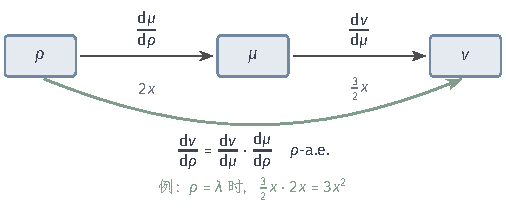
\includegraphics[width=85.651mm]{figures/02-abstract-mathematics/01-metric-and-measure/tikz/c4-chain-rule/figure.pdf}
  \caption{密度的链式规则。箭头表示“箭头终点的测度相对于起点测度的密度”：先从$\rho$换到$\mu$，再从$\mu$换到$\nu$，两段密度相乘就是从$\rho$直接换到$\nu$的密度（绿色弧线），等式在$\rho$几乎处处意义下成立。箭头下方是$[0,1]$上$\rho=\lambda$时的例子，$2x$与$\tfrac32x$相乘得到$3x^2$。}
  \label{fig:dens-chain-rule}
\end{figure}

\paragraph{各因子的几乎处处意义}
$g=\mathrm d\nu/\mathrm d\mu$只确定到$\mu$零测集，而结论是关于$\rho$零测集的。两者并不冲突。设$g'$是$g$的另一个版本，$g\neq g'$只发生在某个$\mu$零测集$M$上，于是乘积$gk$与$g'k$只可能在$M\cap\{k>0\}$上不同。由$0=\mu(M)=\int_Mk\,\mathrm d\rho$，$k$在$M$上$\rho$几乎处处为零，所以$\rho(M\cap\{k>0\})=0$。也就是说，在$k=0$处乘积按约定取$0$，与$g$的取值无关；在$k>0$处，$\mu$的零测例外也是$\rho$的零测例外。无论选哪个版本，乘积都给出同一个$\rho$几乎处处确定的密度。

\subsection{倒数规则}
\label{sec:dens-inverse-rule}

若两个测度相互绝对连续，就可以从任一方换到另一方。反向的密度应当是原密度的倒数，但这需要先保证原密度几乎处处既不为零也不为无穷。

\begin{theorem}[密度的倒数]
\label{thm:dens-inverse}
设$\mu,\nu$是$(X,\mathcal A)$上的$\sigma$有限非负测度，$\nu\ll\mu$且$\mu\ll\nu$，$h=\mathrm d\nu/\mathrm d\mu$。则$0<h<\infty$在$\mu$几乎处处成立，并且
\[
\frac{\mathrm d\mu}{\mathrm d\nu}=\frac1h ,
\]
等式在$\mu$几乎处处意义下成立，也在$\nu$几乎处处意义下成立。
\end{theorem}

\begin{proof}
由Radon–Nikodym定理可取有限值的$h$。令$Z=\{h=0\}$，则$\nu(Z)=\int_Zh\,\mathrm d\mu=0$，由$\mu\ll\nu$得$\mu(Z)=0$，所以$0<h<\infty$在$\mu$几乎处处成立。令$u=1/h$于$X\setminus Z$，$u=0$于$Z$。对任意可测集$A$，由换测度公式，
\[
\int_Au\,\mathrm d\nu=\int_X\mathbf 1_Auh\,\mathrm d\mu=\mu(A\setminus Z)=\mu(A),
\]
所以$u$是$\mu$相对于$\nu$的密度。两个测度等价，零测集相同，因此$\mu$几乎处处与$\nu$几乎处处是同一回事。
\end{proof}

这个结论也可以从链式规则读出：对$\mu\ll\nu\ll\mu$用定理~\ref{thm:dens-chain-rule}，得$(\mathrm d\mu/\mathrm d\nu)\cdot h=\mathrm d\mu/\mathrm d\mu=1$。例如$[0,1]$上$\nu$相对于$\lambda$的密度为$2x$，它只在零测集$\{0\}$上为零，所以$\nu$与$\lambda|_{[0,1]}$等价，反向密度为$1/(2x)$，$x\in(0,1]$。反向密度无界，但仍满足$\int_0^1\frac1{2x}\cdot2x\,\mathrm dx=1=\lambda([0,1])$。

\paragraph{单向绝对连续时的信息丢失}
若只有$\nu\ll\mu$，密度$h$可以在一个正$\mu$测度的区域上为零。取$\mu=\lambda|_{[0,2]}$，$\nu=\lambda|_{[0,1]}$，则$h=\mathbf 1_{[0,1]}$。在正密度区域$\{h>0\}=[0,1]$上，反向表示仍然成立：对$A\subset\{h>0\}$，$\mu(A)=\int_A(1/h)\,\mathrm d\nu$。但在零密度区域$(1,2]$上，$\mu$有质量$1$，$\nu$却为零，无论用什么函数加权，$\int_{(1,2]}u\,\mathrm d\nu$都是$0$，不可能恢复$\mu((1,2])=1$。这时$\mu$并不相对于$\nu$绝对连续，整体的反向密度不存在。图~\ref{fig:dens-one-sided-loss}显示了这块被目标测度完全忽略的区域。

\begin{figure}[!htbp]
  \centering
  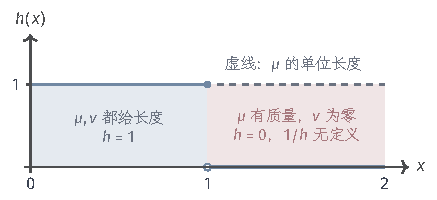
\includegraphics[width=73.914mm]{figures/02-abstract-mathematics/01-metric-and-measure/tikz/c4-one-sided-loss/figure.pdf}
  \caption{单向绝对连续时密度不能取倒数。参考测度$\mu$是$[0,2]$上的长度，目标测度$\nu$是$[0,1]$上的长度，密度$h=\mathbf 1_{[0,1]}$（蓝色实线）。在$[0,1]$上$h=1$，两种测度一致；在红色区域$(1,2]$上$h=0$，$\mu$有质量$1$而$\nu$没有质量，从$\nu$出发无法恢复这部分质量。}
  \label{fig:dens-one-sided-loss}
\end{figure}

一般地，若$\nu\ll\mu$且都$\sigma$有限，令$P=\{h>0\}$，同样的计算给出$\mu(A\cap P)=\int_A\mathbf 1_P/h\,\mathrm d\nu$，即$1/h$是$\mu|_P$相对于$\nu$的密度。原参考测度在零密度区域$X\setminus P$上的质量$\mu|_{X\setminus P}$与$\nu$相互奇异，这正是$\mu$相对于$\nu$的Lebesgue分解中的奇异部分，不能通过相除恢复。倒数公式只能在两个测度等价的范围内整体使用。

\section{密度的计算}
\label{sec:dens-computation}

前几节回答了密度何时存在、怎样使用。本节回到两类具体对象：可数集合上由点质量给出的测度，以及实轴上由累积函数的增量给出的测度。每个例子都按同一顺序处理：先固定参考测度，检查绝对连续性，再求密度，最后代入换测度公式核对它能否恢复目标测度的质量与积分。

\subsection{离散测度的密度}
\label{sec:dens-discrete}

可数集合上每个点都可以单独称量，所以离散测度的密度可以逐点计算，这是向量类比完全成立的情形。需要分别处理的只是参考质量为零的点。

\paragraph{点质量之比}
设$X=\{x_1,x_2,\ldots\}$是可数集合，取全部子集为可测集，参考测度与目标测度分别为
\[
\mu=\sum_im_i\delta_{x_i},\qquad\nu=\sum_ip_i\delta_{x_i},\qquad m_i,p_i\in[0,+\infty).
\]
单点质量有限，可数个单点覆盖$X$，所以两者都$\sigma$有限。

先检查绝对连续。$\mu(A)=0$当且仅当$A$中每点的$m_i$都为零，所以$\nu\ll\mu$当且仅当“$m_i=0$推出$p_i=0$”。在此条件下令
\begin{equation}
h(x_i)=\frac{p_i}{m_i}\quad(m_i>0),\qquad h(x_i)\ \text{取任意非负值}\quad(m_i=0).
\label{eq:dens-discrete}
\end{equation}

对离散测度的积分是加权求和，于是对任意$A\subset X$，
\[
\begin{aligned}
\int_Ah\,\mathrm d\mu&=\sum_{x_i\in A}h(x_i)m_i=\sum_{x_i\in A,\,m_i>0}p_i\\
&=\sum_{x_i\in A}p_i=\nu(A),
\end{aligned}
\]
第三个等号用到$m_i=0$时$p_i=0$。所以$h$是$\nu$相对于$\mu$的密度。

两类点的处理不同。参考质量为正的点上，密度值就是质量之比，被唯一确定。参考质量为零的点构成$\mu$零测集，密度在那里可以任意取值，这正是几乎处处版本在离散情形的样子。以计数测度为参考时所有$m_i=1$，密度就是目标的点质量本身，即概率质量函数。

\paragraph{参考零测点上的目标质量}
若某点$m_i=0$而$p_i>0$，不能用“取一个很大的有限比值”来补救：任何有限或无限的$h(x_i)$都满足$h(x_i)m_i=0\neq p_i$。这时的问题不在于比值难算，而在于$\nu\ll\mu$不成立，密度根本不存在。

正确的做法是先作Lebesgue分解。令$N=\{x_i:m_i=0\}$，则$\nu$的奇异部分与绝对连续部分分别是
\[
\nu_{\mathrm s}=\sum_{x_i\in N}p_i\delta_{x_i},\qquad\nu_{\mathrm{ac}}=\sum_{x_i\notin N}p_i\delta_{x_i} ,
\]
只有$\nu_{\mathrm{ac}}$才有密度$p_i/m_i$。

例如在$X=\{0,1,2\}$上取
\[
\mu=\delta_0+\delta_1,\qquad\nu=\tfrac12\delta_0+\tfrac14\delta_1+\tfrac14\delta_2 ,
\]
则$N=\{2\}$，点$2$上的质量$\tfrac14$是奇异部分。$\nu_{\mathrm{ac}}$的密度在$0,1$处分别为$\tfrac12,\tfrac14$。

\begin{example}[同一分布换两种参考]
\label{ex:dens-poisson}
在$\{0,1,2,\ldots\}$上取参数为$1$的Poisson分布$p_k=\mathrm e^{-1}/k!$为目标。相对于计数测度，密度就是$p_k$本身。若改用几何权重$m_k=2^{-(k+1)}$作参考，所有$m_k>0$，密度为
\[
h(k)=\frac{p_k}{m_k}=\frac{2^{k+1}\mathrm e^{-1}}{k!} .
\]
前六项约为
\[
0.736,\quad1.472,\quad1.472,\quad0.981,\quad0.491,\quad0.196 .
\]
核对集合$\{0,1\}$的质量。直接求和与加权求和分别是
\[
\begin{aligned}
\nu(\{0,1\})&=2\mathrm e^{-1}\approx0.7358,\\
h(0)m_0+h(1)m_1&\approx0.7358\cdot0.5+1.4715\cdot0.25\approx0.7358 ,
\end{aligned}
\]
两者一致。两种密度由链式规则联系：几何权重相对于计数测度的密度是$m_k$，所以$h(k)\cdot m_k=p_k$。
\end{example}

图~\ref{fig:dens-discrete}画出了两组点质量及它们的比值。比值大于$1$的地方，目标比参考更重；$k$增大后几何权重比阶乘倒数衰减得慢，比值趋于零。

\begin{BookInlineFigure}
  \centering
  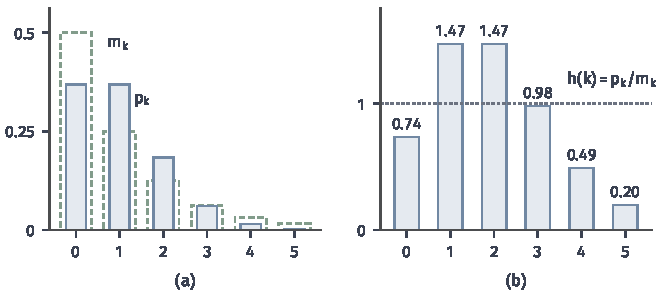
\includegraphics[width=112mm]{figures/04-spaces-measures-and-geometry/02-measure/matplotlib/dens-discrete/figure.pdf}
  \caption{可数集合上的离散密度。(a)绿色虚线框为几何参考质量$m_k=2^{-(k+1)}$，蓝色柱为Poisson目标质量$p_k=\mathrm e^{-1}/k!$，$k=0,\ldots,5$。(b)密度$h(k)=p_k/m_k$：$k=1,2$处目标质量相对参考最多，$h$约为$1.47$；$k$增大后$h$趋于零。}
  \label{fig:dens-discrete}
\end{BookInlineFigure}

密度的计算与总质量是否有限无关。仍以几何权重为参考，计数测度$\sum_k\delta_k$的密度是$h(k)=2^{k+1}$，目标的总质量为$+\infty$，但每个集合上的质量都由$h$正确恢复。代入换测度公式，例如对$f(k)=k$，
\[
\sum_kk\,p_k=\sum_kk\,\frac{p_k}{m_k}\,m_k ,
\]
两边都是Poisson分布的均值$1$。

\subsection{由累积函数求密度}
\label{sec:dens-cumulative-density}

实轴上的测度常常由累积函数给出。设$F:\mathbb R\to\mathbb R$单调不减且右连续，第~\ref{chap:measure}章的Stieltjes构造给出Borel测度$\mu_F$，满足$\mu_F((s,t])=F(t)-F(s)$。它在每个有界区间上有限，因而$\sigma$有限。我们要问$\mu_F$何时有Lebesgue密度，以及密度怎样从$F$算出。

\begin{theorem}[累积函数的密度]
\label{thm:dens-cumulative}
设$F:\mathbb R\to\mathbb R$单调不减且右连续。
\begin{enumerate}
\item 若$F$在每个有界闭区间上绝对连续，则$\mu_F\ll\lambda$，并且
\begin{equation}
\frac{\mathrm d\mu_F}{\mathrm d\lambda}=F'\qquad\lambda\text{几乎处处}.
\label{eq:dens-cumulative}
\end{equation}
\item 反之，若$\mu_F\ll\lambda$，则$F$在每个有界闭区间上绝对连续。
\end{enumerate}
\end{theorem}

\begin{proof}
(1) 由第~\ref{chap:integration}章，绝对连续函数几乎处处可导，导数局部可积，并且
\[
F(t)-F(s)=\int_s^tF'(x)\,\mathrm dx .
\]
$F$单调不减，在可导点差商非负，所以$F'\geq0$几乎处处，可以取非负版本。

令$\nu(A)=\int_AF'\,\mathrm d\lambda$。由定理~\ref{thm:dens-weighted-measure}它是测度，并且在每个区间$(s,t]$上与$\mu_F$相等。两者在每个$(-m,m]$上有限；半开区间族对交封闭并生成Borel $\sigma$代数，由第~\ref{chap:measure}章测度延拓的唯一性，$\nu=\mu_F$。于是$F'$是$\mu_F$相对于$\lambda$的密度，$\mu_F\ll\lambda$。

(2) 固定$[a,b]$。$\lambda$是$\sigma$有限的，由Radon–Nikodym定理存在非负可测$h$使$\mu_F(A)=\int_Ah\,\mathrm d\lambda$，并且
\[
\int_a^bh\,\mathrm dx=F(b)-F(a)<\infty .
\]
于是对$x\in[a,b]$，
\[
F(x)=F(a)+\mu_F((a,x])=F(a)+\int_a^xh(t)\,\mathrm dt .
\]
可积函数的变上限积分绝对连续，所以$F$在$[a,b]$上绝对连续。
\end{proof}

定理把函数的绝对连续与测度的绝对连续联系起来：对单调累积函数，“总长度小的区间组上增量之和小”恰好对应“长度零测集上没有增量质量”。密度就是导数，但只在几乎处处意义下确定：$F$在个别点上可以没有导数，在那里给密度取什么值都不影响$\mu_F$。

\begin{example}[多项式累积函数]
\label{ex:dens-square-cdf}
令$F(x)=0$（$x<0$），$F(x)=x^2$（$0\leq x\leq1$），$F(x)=1$（$x>1$）。$F$在每个有界闭区间上是Lipschitz的，因而绝对连续，于是$\mu_F$相对于$\lambda$的密度是
\[
F'(x)=2x\mathbf 1_{(0,1)}(x).
\]
在$x=1$处$F$没有导数，但单点不影响密度。代入换测度公式，
\[
\int x\,\mathrm d\mu_F=\int_0^1x\cdot2x\,\mathrm dx=\tfrac23 ,
\]
与第~\ref{sec:dens-change-of-measure}小节的例子一致。
\end{example}

\paragraph{检查原子与奇异连续部分}
定理的条件不能省略，也不能只检查$F$是否连续。计算一般累积函数的密度时，应当按第~\ref{sec:dens-decomposition}节的分解逐项检查。第一步读出跳跃：由式~\eqref{eq:dens-jump}的同一推导，$F(x)-F(x-)=\mu_F(\{x\})$，跳跃点就是原子。第二步去掉跳跃后检查余下的连续部分是否绝对连续；若是，它的导数就是$\mu_F$的绝对连续部分的密度，否则还有奇异连续部分。只把$F'$当作整个测度的密度，会同时漏掉这两类质量。

\begin{example}[有跳跃的累积函数]
\label{ex:dens-mixed-cdf}
令
\[
F(x)=\begin{cases}0,&x<0,\\\tfrac12+\tfrac x2,&0\leq x<1,\\1,&x\geq1.\end{cases}
\]
$F$在$0$处从$0$跳到$\tfrac12$，其余处连续，所以$\mu_F$有原子$0$，质量$\tfrac12$。去掉跳跃后的$F-\tfrac12\mathbf 1_{[0,\infty)}$在$[0,1]$上是$\tfrac x2$，绝对连续，导数$\tfrac12$。于是
\[
\mu_F=\tfrac12\delta_0+\tfrac12\lambda|_{[0,1]} ,
\]
只有后一项有Lebesgue密度$\tfrac12\mathbf 1_{[0,1]}$。

用换测度公式检验差别。取$g(x)=1+x$，正确的积分把原子和密度两部分都算上：
\[
\int g\,\mathrm d\mu_F=\tfrac12g(0)+\int_0^1\tfrac12(1+x)\,\mathrm dx=\tfrac12+\tfrac34=\tfrac54 .
\]
若误把$F'$当作整个测度的密度，只得到
\[
\int_0^1(1+x)\cdot\tfrac12\,\mathrm dx=\tfrac34 ,
\]
恰好漏掉原子贡献的$\tfrac12g(0)=\tfrac12$。
\end{example}

图~\ref{fig:dens-cumulative-jump}左边是累积函数，右边是它对应的测度。左图的跳跃高度变成右图的箭头，左图的斜率变成右图的密度。

\begin{BookInlineFigure}
  \centering
  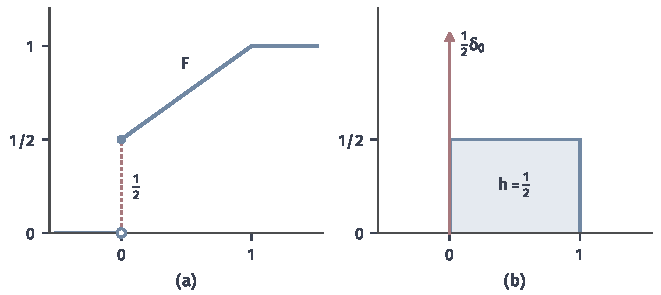
\includegraphics[width=112mm]{figures/04-spaces-measures-and-geometry/02-measure/matplotlib/dens-cumulative-jump/figure.pdf}
  \caption{有跳跃的累积函数与它的测度。(a)$F$在$0$处跳跃$\tfrac12$（红色虚线），在$(0,1)$上斜率为$\tfrac12$。(b)对应的测度$\mu_F=\tfrac12\delta_0+\tfrac12\lambda|_{[0,1]}$：红色箭头是原子，蓝色区域是密度$\tfrac12$表示的连续质量。}
  \label{fig:dens-cumulative-jump}
\end{BookInlineFigure}

连续却不绝对连续的情形由Cantor函数给出。第~\ref{sec:dens-real-line-decomposition}小节的混合例子中，去掉跳跃后的$\tfrac x2+\tfrac14F_C(x)$已经连续，却仍有$\tfrac14$的奇异连续质量，其导数几乎处处等于$\tfrac12$，只恢复绝对连续部分。所以“$F$连续”“$F$几乎处处可导”都不足以让导数成为整个测度的密度，必须要求绝对连续。

对右连续的有界变差函数，增量可以为负。这时可以先写成两个单调函数之差，再对两个Stieltjes测度分别应用本小节的步骤，最后按有限有符号测度的规则相减。

\section{本章小结}
\label{sec:dens-summary}

本章开头问：一个测度何时能写成参考测度的加权积分，权重怎样计算，有了权重之后积分怎样改写。全章可以对照有限点集上的向量来读，表~\ref{tab:dens-vector-analogy}列出了对应关系，以及类比失效之后一般情形用什么代替。

\begin{BookInlineTable}
\small
\begin{tabular}{@{}>{\RaggedRight\arraybackslash}p{22mm}>{\RaggedRight\arraybackslash}p{\dimexpr(\linewidth-22mm-4\tabcolsep)*2/5\relax}>{\RaggedRight\arraybackslash}p{\dimexpr(\linewidth-22mm-4\tabcolsep)*3/5\relax}@{}}
\toprule
概念 & 有限点集上的向量 & 一般测度\\
\midrule
测度 & 非负向量 & 集合上的可数可加函数\\
绝对连续 & 零分量位置的包含 & 对每个可测集检查零测关系\\
相互奇异 & 两向量无公共正分量 & 用一个可测集分开，闭支撑可以相交\\
密度 & 逐分量比值 & 无逐点比值，由集合上的积分等式确定\\
Lebesgue分解 & 按$m_i>0$与否分下标 & 寻找承载最多质量的零测集\\
换参考 & 对角矩阵乘向量 & 换测度公式\\
连续换参考 & 对角矩阵相乘 & 链式规则，几乎处处成立\\
对调参考与目标 & 对角矩阵求逆 & 倒数规则，要求两个测度等价\\
\bottomrule
\end{tabular}
\caption{密度理论的向量类比。}
\label{tab:dens-vector-analogy}
\end{BookInlineTable}

回答从零测集开始。绝对连续$\nu\ll\mu$要求参考测度忽略的集合目标测度也忽略，它有方向，而且必须对每个可测集检查，单点检查在不可数集合上不够。相互奇异$\mu\perp\nu$要求一个可测集把两种质量完全分开，闭支撑相交的两个测度仍可以相互奇异。

加权方向总是可行的：任给非负可测权重，对参考测度积分就得到一个测度，并且它相对于参考绝对连续。反方向由Radon–Nikodym定理回答：两个测度都$\sigma$有限时，$\nu\ll\mu$保证密度存在，密度在$\mu$几乎处处意义下唯一。证明取所有不超过目标的权重中积分最大的一个，Hahn分解说明剩余质量只能为零。计数测度的反例说明参考测度的$\sigma$有限性不能随意去掉；有限有符号测度则对两个变差分别求密度，得到一个可积密度，其正负部对应Jordan分解。

一般的测度未必绝对连续。Lebesgue分解把它唯一地拆成绝对连续部分与奇异部分：构造依靠承载最多质量的零测集，唯一性只读取两个集合上的值，密度表示再用Radon–Nikodym定理。实轴上以长度为参考时，奇异部分又分成原子与奇异连续部分。累积函数的跳跃读出原子，Cantor测度说明连续的累积函数仍可以把全部质量放在长度为零的集合上，普通导数只恢复绝对连续部分的密度。

有了密度，换测度公式把$\int f\,\mathrm d\nu$改写成$\int fh\,\mathrm d\mu$：点和被积函数都不变，只是累计权重乘上$h$。相对同一参考的密度可以非负组合，带符号的组合需要有限性。逐次换参考时密度相乘，各因子的零测例外最终都是底层参考的零测例外。两个测度等价时密度可以取倒数，单向绝对连续时只能在正密度区域上取倒数，零密度区域上的参考质量无法恢复。

具体计算时先查绝对连续，再求密度。离散测度的密度是参考质量为正处的点质量之比，参考零测点上若仍有目标质量，密度不存在，应先分出奇异部分。实轴上单调累积函数绝对连续时，导数就是密度；一般情形先读出跳跃，再检查去掉跳跃后的部分是否绝对连续。本章的所有运算都在同一个空间上进行；下一章研究质量沿可测映射从一个空间转移到另一个空间，那时目标空间上的密度要结合本章的换测度公式与坐标换元来计算。

